\documentclass{article}
\usepackage{graphicx} % Required for inserting images
\usepackage{amsmath}
\usepackage{tikz}
\usetikzlibrary{automata, positioning, arrows.meta}
\title{mini project}
\author{j.poulard Y.Chen }
\date{October 2026}

\begin{document}

\maketitle

\section{Introduction}
\section{Physical Modelling}
Hi Julia, once you have the print-head velocity expressions or simulation results from Q1.4, could you share them with me? I’ll use them to calculate the deposition speed for Q1.6.

\subsection*{Q1.5: Nozzle Model}
Inductor: $L_n$ \\ Resistor: $R_n$ \\Capacitor: $C_n$
\\resistor voltage: $v_c$ \\capacitor voltage: $v_c$, since capacitor and resistor are connected in parallel
\paragraph{modelling assumptions}
\begin{itemize}
\item uniform nozzle temperature $T_n(t)$
\item constant electrical and thermal parameters
\item combined heat loss to the environment and filament
\item all ell electrical power dissipated in $R_n$ is transferred to the nozzle as heat.
\end{itemize}

\paragraph{variables and sign conventions}
\begin{itemize}
\item inductor current $i_L=i_n$, the positive direction of $i_n$ is from the input terminal towards the parallel branches. The voltage $v_c$ is defined as the potential of the upper node relative to the lower node.
\end{itemize}

inductor voltage drop:$v_L$
\begin{equation}v_L=L_n\dot{i}_n\end{equation}
the nozzle voltage: 
\begin{equation}u_n=v_L+v_c\end{equation}
the inductor current change rate:\begin{equation}\dot{i}_n=\frac{1}{L_n}\left(u_n-v_c\right)\label{eq:inductor current change rate}\end{equation}
inductor current: $i_n$\\
\begin{equation}i_n=i_c+i_R\end{equation}
resistor current: $i_R$
\begin{equation}i_R=\frac{v_c}{R_n}\end{equation}
therefore, \begin{equation}i_n=C_n\dot{v}_c+\frac{v_c}{R_n}\end{equation}
capacitor voltage change rate: \begin{equation}\dot{v}_c=\frac{1}{C_n}\left({i_n}-\frac{v_c}{R_n}\right)\label{eq:capacitor voltage change rate}\end{equation}
heating power of resistor \begin{equation}P=\frac{v_c^2}{R_n}\end{equation}
nozzle thermal losses: \begin{equation}P_\mathrm{loss}=\frac{T_n-T_e}{R_{t,n}}\end{equation}
thermal energy \begin{equation}\dot{Q}=P-P_\mathrm{loss}\end{equation}
temperature change rate \begin{equation}
\dot{T}_n=\frac{P-P_\mathrm{loss}}{C_{t,n}}\end{equation}
\begin{equation}
\dot{T}_n=\frac{1}{C_{t,n}}\left(\frac{v_c^2}{R_n}-\frac{T_n-T_e}{R_{t,n}}\right)\label{eq:temperature change rate}\end{equation}
since three differential equation equation~\eqref{eq:inductor current change rate}, ~\eqref{eq:capacitor voltage change rate},~\eqref{eq:temperature change rate}
the state-space description of the form $\dot{x}_n=f_n\left(x_n,u_n\right)$ goes to $x_n=[{T_n},{i_n},{v_c}]^\top$
\begin{equation}
\dot{x}_n=
\begin{bmatrix}
    \dot{T}_n\\
    \dot{i}_n\\
    \dot{v}_c
\end{bmatrix}=
\begin{bmatrix}
    \frac{1}{C_{t,n}}\left(\frac{v_c^2}{R_n}-\frac{T_n-T_e}{R_{t,n}}\right)\\
    \frac{1}{L_n}\left(u_n-v_c\right)\\
    \frac{1}{C_n}\left({i_n}-\frac{v_c}{R_n}\right)
\end{bmatrix}
\end{equation}





\subsection*{Q1.6: Filament Cooling Model}
\paragraph{geometry and modeling assumptions}
Following the problem statement, the printed filament is assumed to have a square cross-section, with its lower face in contact with the heated plate. Consider a small segment of length $\Delta s$ along the filament path, with cross-sectional side length $a$. The filament temperature is denoted by $T(s,t)$ and is assumed to be uniform across each cross-section. At deposition, the filament temperature is assumed to equal the nozzle temperature.
\begin{equation}V=a^2\Delta s\end{equation}


\paragraph{thermal energy balance}
thermal energy accumulation rate:
\begin{equation}
\dot{E}
=c_p m \frac{\partial T}{\partial t}
=c_p \rho a^2 \Delta s
 \frac{\partial T}{\partial t}
\label{eq: Edot}
\end{equation}
three heat transfer paths are:
filament-air: convection
filament-plate: conduction
filament-filament: conduction
the area contact to the plate and air
\begin{equation}
A_b=a\Delta s
\qquad
A_{\mathrm{air}}=3a\Delta s
\end{equation}
so firstly the convective heat transfer from the filament to air ($h_{air}$ is the heat transfer coefficient of air):
\begin{equation}
P_{air}
=h_{air} A_{air} (T(s,t)-T_e)
=h_{air} 3a \Delta s (T(s,t)-T_e)
\label{eq: Pair}
\end{equation}
secondly, heat conduction between the filament and the plate is modelled using the effective thermal contact conductance per unit area $h_b$, $T_b$ is the print bed temperature: 
\begin{equation}
P_b
=h_b A_b (T_b-T(s,t))
=h_b a \Delta s (T_b-T(s,t))
\label{eq:Pb}
\end{equation}
lastly, consider heat conduction along the filament between adjacent segments. For a segment extending from $s$ to $s+\Delta s$, define $P_{\mathrm{cond}}(s,t)$ as the heat transfer rate in the positive $s$ direction:
\begin{equation}
P_{\mathrm{cond}}
=- k \frac{\partial T}{\partial s} A
\end{equation}
\begin{equation}
P_f
=P_{\mathrm{cond}}(s,t)-P_{\mathrm{cond}}(s+\Delta s,t)
=-k a^2 (\frac{\partial T}{\partial s} (s,t) -\frac{\partial T}{\partial s}(s+\Delta s,t))
\label{eq: Pcond}
\end{equation}
dividing both sides by $\Delta s$ gives:
\begin{equation}
\frac {P_f}{\Delta s}= k a^2 \frac{\frac{\partial T}{\partial s} (s+\Delta s,t) -\frac{\partial T}{\partial s}(s,t)}{\Delta s}
\end{equation}
Taking the limit as $\Delta s\to 0$ gives:
\begin{equation}
\lim_{\Delta s \to 0}\frac{P_f}{\Delta s}= ka^2
\frac{\partial}{\partial s}
\left(\frac{\partial T}{\partial s}\right)
=ka^2\frac{\partial^2 T}{\partial s^2}
\end{equation}
According the energy conservation, the heat accumulated is equal to the heat came into the system, therefore,
\begin{equation}
\dot {E} =-P_{air}+P_b+P_f
\label{eq:eb}
\end{equation}
divide both sides by $\Delta s$, according to ~\eqref{eq: Edot}, ~\eqref{eq: Pair}, ~\eqref{eq:Pb}, and ~\eqref{eq: Pcond}:
\begin{equation}
c_p \rho a^2 \frac{\partial T}{\partial t}
=-h_{air} 3a (T(s,t)-T_e)+h_b a (T_b-T(s,t))+ka^2\frac{\partial^2 T}{\partial s^2}
\label{eq:energybalance}
\end{equation}
divide both side by $c_p\rho a^2$:
\begin{equation}
\frac{\partial T}{\partial t}
= -\frac{3h_{air}}{c_p\rho a}(T-T_e)
 +\frac{h_b}{c_p\rho a}(T_b-T)
 +\frac{k}{c_p \rho}\frac{\partial^2 T}{\partial s^2}
 \end{equation}

\paragraph{growing domain and deposition condition}

During printing, filament is assumed to be deposited continuously along the path. the speed of the print head along the path is 
\begin{equation}
v_p(t)=\sqrt{\dot{x}(t)^2+\dot{y}(t)^2}
\end{equation}
Allowing for a time-varying printing speed, the deposited length is 
\begin{equation}
l(t)=\int_0^tv_p(\tau)\,\mathrm{d}\tau,
\qquad
0\le t\le t_{\mathrm{end}}.
\end{equation}
Printing ends when $l(t_{\mathrm{end}})=L$.
For $t>t_{\mathrm{end}}$, the deposited length remains $L$. 
\paragraph{Boundary conditions during and after printing}(define how the continuous temperature state connect with the environment and the filament)
Let $L$ denote the total length of the  printing path and $l(t)$ the length of filament deposited by time $t$.
The temperature equation applies only to $0<s<l(t)$ , where $s=0$ is the starting position of the printing path and $s=l(t)$ is the current deposition front.
The temperature of newly deposited filament is assumed to equal the nozzle temperature $T_n(t)$:
\begin{equation}
T(l(t),t)= T_n(t),
\qquad
0<t<t_{\mathrm{end}}
\end{equation}
After printing is complete, the starting and ending faces at $s=0$ and $s=L$ meet at a zero-thickness interface. We assume perfect thermal contact, with no thermal contact resistance. We also neglect energy storage and any separate heat loss at the interface. The two ends therefore exchange heat by conduction, as other adjacent filament segments do. The positive $s$ direction is defined along the filament path from the starting point towards the deposition front. At $s=0$, outward heat flow is in the negative $s$ direction. With heat flow defined in the positive $s$ direction, $P_{\mathrm{cond}}(L,t)$ enters the interface and $P_{\mathrm{cond}}(0,t)$ leaves it. Conservation of energy therefore requires continuity of the heat-transfer rate:
\begin{equation}
P_{\mathrm{cond}}(L,t)=P_{\mathrm{cond}}(0,t),
\qquad
t>t_{\mathrm{end}}
\end{equation}
consider the zero-thickness starting end face with area $a^2$. Its temperature is $T(0,t)$, and the ambient air temperature is $T_e$.

Heat is conducted from the deposited filament immediately adjacent to the starting end face towards that face, and is then transferred to the surrounding air by convection. Since the starting end face is modelled as a zero-thickness surface with no energy storage, the net conductive heat-transfer rate into the face equals the net convective heat-transfer rate from the face to the air. 
The outward heat-transfer rate is 
\begin{equation}
P_{\mathrm{end,out}}=
h_{\mathrm{air}} a^2 \bigl(T(0,t)-T_e\bigr)
\end{equation}
The positive $s$ direction is defined along the filament path from the starting point towards the deposition front. At $s=0$, outward heat flow is in the negative $s$ direction.
\begin{equation}
P_{\mathrm{end,out}}=-P_{\mathrm{cond}}(0,t)
\end{equation}
Using Fourier's law, the boundary condition at the starting end face is
\begin{equation}
k \frac{\partial T}{\partial s}(0,t)
=h_{\mathrm{air}} \bigl(T(0,t)-T_e\bigr)
\qquad
0<t<t_{\mathrm{end}}
\end{equation}
Under the assumption of perfect thermal contact, the two sides of the closure interface, located at $s=0$ and $s=L$, have the same temperature, i.e., there is no temperature jump across the interface:
\begin{equation}
T(0,t)=T(L,t),
\qquad t>t_{\mathrm{end}}
\end{equation}
Perfect thermal contact means that the interface introduces no additional thermal resistance, so there is no temperature jump across it. this does not imply the adjacent filament segments have the same average temperature.
\paragraph{numerical method}
We use the finite volume method and divide the deposited filament into cells of finite length. For the $i$-th cell, the left and right boundaries are located at $s_{i-1/2}$ and $s_{i+1/2}$,respectively.
The cell length is
\begin{equation}
\Delta s_i 
=s_{i+1/2}-s_{i-1/2}
\end{equation}
the cell-average temperature is defined as
\begin{equation}
T_i(t)=\frac{1}{\Delta s_i}\int_{s_{i-1/2}}^{s_{i+1/2}}{T(s,t)}\,\mathrm{d}s
\end{equation}
Here, $T_i(t)$ represents the average temperature of the cell; it does not imply that the actual temperature is uniform throughout the cell. The density $\rho$, specific heat capacity $c_p$, and cross-sectional side length $a$ are assumed to be constant. 
For two adjacent deposited cells, the distance between their center is 
\begin{equation}
d_{i,i+1}=\frac{\Delta s_i+\Delta s_{i+1}}{2}
\end{equation}
Using the cell-average temperatures to approximate the temperatures at the cell center, the temperature gradient at their shared boundary is approximated by
\begin{equation}
\left.\frac{\partial T}{\partial s}\right|_{s_{i+1/2}}
\approx \frac{T_{i+1}-T_i}{d_{i,i+1}}
\end{equation}
Substituting this approximation into Fourier's law gives the conductive heat-transfer rate across the shared boundary:
\begin{equation}
    P_{i+1/2}
    \approx -ka^2\frac{T_{i+1}-T_i}{d_{i,i+1}}
\end{equation}
where $P_{i+1/2}$ is defined as positive in the positive $s$ direction.
Applying the energy balance in ~\eqref{eq:eb} to an already deposited interior cell of fixed length gives
\begin{equation}
\begin{aligned}
\rho c_p a^2 \Delta s_i \frac{\mathrm{d}T_i}{\mathrm{d}t}
= {}&-3h_{\mathrm{air}}a\Delta s_i(T_i-T_e)\\
  &+h_b a\Delta s_i(T_b-T_i) \\
  {}&+  P_{i-1/2}-P_{i+1/2}
\end{aligned}
\end{equation}
For uniformly spaced cells of length $\Delta s$, the distances between adjacent cell centers are also $\Delta s$. Substituting the conductive heat-transfer approximations and dividing by the cell thermal capacity $\rho c_p a^2 \Delta s$ gives
\begin{equation}
    \begin{aligned}
        \frac{\mathrm{d}T_i}{\mathrm{d}t}
        ={}&-\frac{3h_{\mathrm{air}}}{\rho c_p a}(T_i-T_e)\\
           &+\frac{h_b}{\rho c_p a}(T_b-T_i)\\
           &+ \frac{k}{\rho c_p(\Delta s)^2}
           \left(T_{i-1}-2T_i+T_{i+1}\right)\\
    \end{aligned}
    \label{eq:interiorcell}
\end{equation}
This provides a finite-volume spatial discretisation of ~\eqref{eq:energybalance} for fixed-length interior cells on a uniform grid, with deposited neighbouring cells on both sides.
During printing, the starting end face loses heat to the air by convection. To express this heat-transfer rate in terms of the first cell-average temperature $T_1$, let $T_s=T(0,t)$ denote the starting-end surface temperature. Consider a first cell of fixed length $\Delta s$.
The distance from its center to the starting end face is $\Delta s/2$.
Using $T_1$ to approximate the temperature at the cell centre, the temperature gradient at the starting end is approximated by
\begin{equation}
    \frac{\partial T}{\partial s}(0,t)
    \approx \frac{T_1-T_s}{\Delta s/2}.
\end{equation}

Since $P_{\mathrm{cond}}$ is positive in the positive $s$ direction, whereas $P_{\mathrm{end,out}}$ is positive outwards at $s=0$, Fourier's law gives
\begin{equation}
    P_{\mathrm{end,out}}
    =-P_{\mathrm{cond}}(0,t)
    \approx \frac{2ka^2}{\Delta s }(T_1-T_s)
\end{equation}
The end face has no independent energy storage, so the conductive heat-transfer rate into the face equals the convective heat-transfer rate from the face to the air. Equating these rates within the discrete approximation gives 
\begin{equation}
    \frac{2ka^2}{\Delta s}(T_1-T_s)
    =h_{\mathrm{air}}a^2(T_s-T_e)
\end{equation}
cancelling $a^2$ and collecting the terms containing $T_s$ yields
\begin{equation}
    \left(\frac{2k}{\Delta s}+h_{\mathrm{air}}\right)T_s
    =\frac{2k}{\Delta s}T_1+h_{\mathrm{air}}T_e
\end{equation}
Therefore,
\begin{equation}
    T_s=
    \frac{\dfrac{2k}{\Delta s}T_1+h_{\mathrm{air}}T_e}
    {\dfrac{2k}{\Delta s}+h_{\mathrm{air}}}
\end{equation}
Subtracting $T_e$ gives
\begin{equation}
    \begin{aligned}
        T_s-T_e
        &=
        \frac{
        \dfrac{2k}{\Delta s}T_1+h_{\mathrm{air}}T_e
        -\left(\dfrac{2k}{\Delta s}+h_{\mathrm{air}}\right)T_e
        }{
        \dfrac{2k}{\Delta s}+h_{\mathrm{air}}
        }\\
        &=
        \frac{T_1-T_e}
        {1+\dfrac{h_{\mathrm{air}}\Delta s}{2k}}
    \end{aligned}
\end{equation}
Substituting this expression into the convection law gives the discrete starting-end heat-transfer rate:
\begin{equation}
    P_{\mathrm{end,out}}
    =
    \frac{h_{\mathrm{air}}a^2}
    {1+\dfrac{h_{\mathrm{air}}\Delta s}{2k}}
    (T_1-T_e)
    \label{eq:endheatloss}
\end{equation}
This expression applies while the starting end face is exposed to air during printing and the first cell has the fixed length $\Delta s$.
\\for a interior cell $\Delta s$
\\During printing, once the first two cells have reached the fixed length $\Delta s$, applying the energy balance in ~\eqref{eq:eb} to the first cell and using ~\eqref{eq:endheatloss} gives
\begin{equation}
    \begin{aligned}
        \frac{\mathrm{d}T_1}{\mathrm{d}t}
        =
        &+\frac{h_b}{\rho c_p a}(T_b-T_1)\\
        &-\frac{3h_{\mathrm{air}}}{\rho c_p a}(T_1-T_e)\\
        &+\frac{k}{\rho c_p(\Delta s)^2}(T_2-T_1)\\
        &-\frac{h_{\mathrm{air}}}
        {\rho c_p\Delta s
        \left(1+\dfrac{h_{\mathrm{air}}\Delta s}{2k}\right)}
        (T_1-T_e)\\
    \end{aligned}
    \label{eq:firstcell}
\end{equation}
The four terms represent heat transfer from the plate, convective heat loss through the three exposed lateral faces, conduction from the neighbouring second cell, and convective heat loss through the starting end face, respectively.
\\the growing cell
\\Depositing enough filament to fill one cell takes a finite amount of time. During this interval, the material already deposited within the cell exchanges heat with the air and the plate, while new material enters at the nozzle temperature $T_n(t)$.
\\Therefore, the cell-average temperature is affected both by heat exchange and by the addition of new material. We describe the evolution of the average temperature $T_N(t)$ of the currently growing cell, where $N$ denotes its index and $T_n(t)$ denotes the nozzle temperature.
\begin{equation}
    \ell_N(t)=l(t)-(N-1)\Delta s,
    \qquad
    0<\ell_N<\Delta s
\end{equation}
\begin{equation}
    m_N=\rho a^2 \ell_n
    \qquad
    \dot{m}_N=\rho a^2 v_p
\end{equation}
the energy input 
\begin{equation}
    P=\dot{m}_Nc_p(T_n-T_e)
\end{equation}
Let $Q_N$ denote the net heat transfer rate into the growing cell through its left and right boundaries, its contact with the plate, and convection with the air.
 It excludes the energy carried by newly deposited material.
\begin{equation}
    \frac{\mathrm{d}}{\mathrm{d}t}[m_Nc_p(T_N-T_e)]=Q_N+\dot{m}_Nc_p(T_n-T_e)
\end{equation}
therefore,
\begin{equation}
    \dot{T}_N=
    \frac{Q_N}{\rho c_p a^2 \ell_N}
    +\frac{v_p}{\ell_N}(T_n-T_N)
    \qquad
    l_N>0
\end{equation}
\\nearly uniform
To assess spatial uniformity after printing is complete, we use the average temperature of entire ring as reference temperature. For $M$ equal-length cells,
\begin{equation}
    T_\mathrm{ref}(t)=
    \frac{1}{M}\sum_{i=1}^{M} T_i(t),
\end{equation}
The temperature is considered nearly uniform when
\begin{equation}
    \max_{1\le i\le M}
    \left|T_i(t)-T_{\mathrm{ref}}(t)\right|
    \le 0.05\, \mathrm{K},
    \qquad t\ge t_{\mathrm{end}}
\end{equation}
\begin{equation}
    \Delta T_{\mathrm{spread}}(t)<\epsilon_T
\end{equation}



\section{Finite State Machine}
\subsection*{Q2.1: Filament Replacement}
the event $C$ denotes a request to print a new colour, while the event $F$ indicates that the spool currently in use has run out of filament.
\\Transition labels follow the format ``event/action''. 
The coordinates $(x_p,y_p)$ denote the wipe-tower location. The machine remains in its current state until the corresponding transition event occurs. 
Nozzle heating remains enabled during heating up and the return to the saved position.
\begin{figure}[htbp]
    \centering
    \resizebox{\linewidth}{!}{%}
        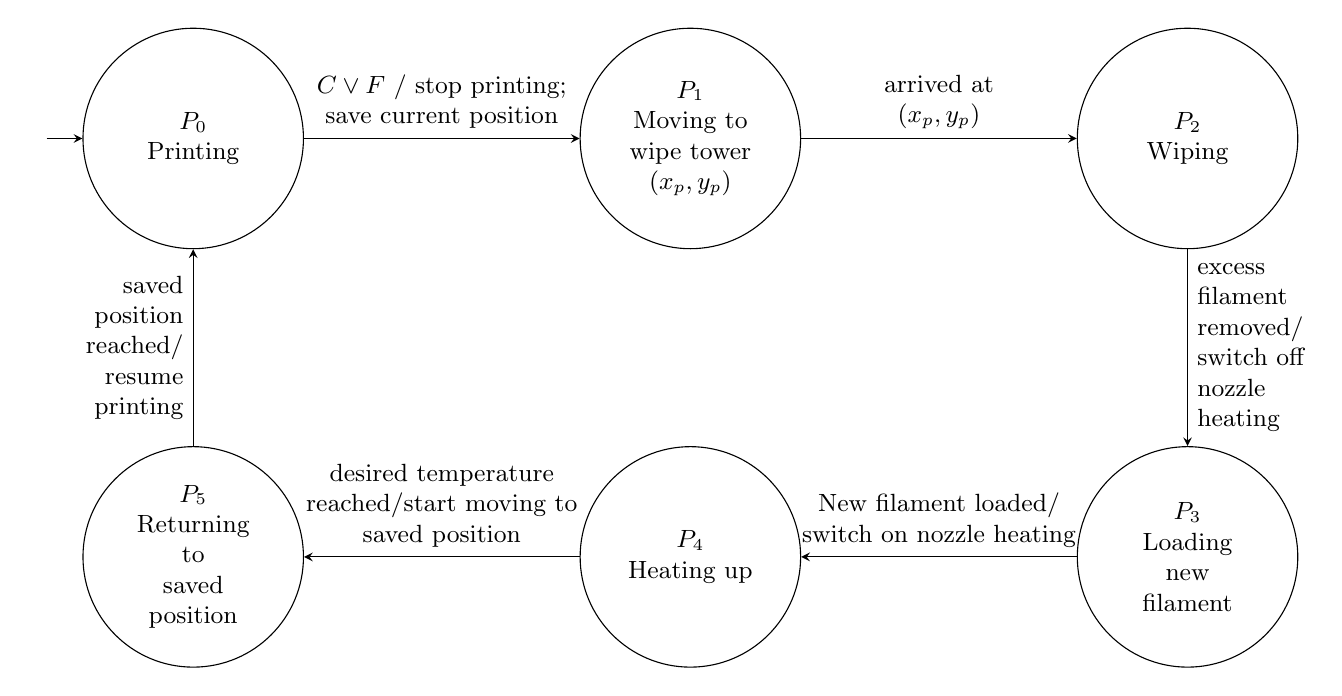
\begin{tikzpicture}[
        >=stealth,
        every state/.style={
        minimum size=2.8cm,
        text width =1.8cm,
        align=center,
        inner sep=0pt,
      font=\small
        },
        initial text={}
    ]
        \node[state,initial](p0){$P_0$\\Printing};
        \node[state,right=3.5cm of p0](p1)
        {$P_1$\\Moving to\\wipe tower\\$(x_p,y_p)$};
        \draw[->](p0)--node[above,align=center, font=\small]
        {$C \lor F$ / stop printing;\\save current position}
        (p1);
        \node[state,right=3.5cm of p1](p2)
        {$P_2$\\Wiping};
        \draw[->](p1)--
        node[above,align=center,
        font=\small]
        {arrived at\\$(x_p,y_p)$}
        (p2);
        \node[state,below=2.5cm of p2](p3)
        {$P_3$\\Loading new\\filament};
        \draw[->](p2)--node[right,align=left,font=\small]
        {excess\\filament \\removed/\\switch off \\nozzle\\heating}
        (p3);
        \node[state,left=3.5cm of p3](p4)
        {$P_4$\\Heating up};
        \draw[->](p3)--node[above,align=center,font=\small]
        {New filament loaded/\\switch on nozzle heating}
        (p4);
        \node[state, left=3.5cm of p4](p5)
        {$P_5$\\Returning to\\saved position};
        \draw[->](p4)--node[above, align=center, font=\small]
        {desired temperature\\ reached/start moving to\\ saved position}
        (p5);
        \draw[->](p5)--node[left,align=right,font=\small]
        {saved\\position\\ reached/\\resume\\printing}
        (p0);
    \end{tikzpicture}%
    }
    \caption{finite-state machine for filament replacement.}
    \label{fig:filament-fsm}
\end{figure}




\end{document}
